\label{lab:corrMvt}

\section{Introduction}

Nous allons maintenant présenter les techniques de correction du mouvement respiratoire proposées dans la littérature. 

Deux approches existent pour la correction du mouvement : les techniques dites prospectives, qui consistent à réaliser la correction pendant l'acquisition en sélectionnant les données à conserver, et rétrospectives, qui réalisent la correction \textit{a posteriori}, après l'acquisition des données. Actuellement, les techniques les plus prometteuses sont rétrospectives, car elles permettent d'utiliser l'ensemble des données du cycle respiratoire.

\section{Synchronisation respiratoire}

La synchronisation respiratoire correspond à un découpage du cycle respiratoire selon la phase (voir figure~\ref{fig:gatingRespi}) ou l'amplitude (voir figure~\ref{fig:gatingRespiAmplitude}). Une seule des phases ou amplitude sera sélectionnée pour la reconstruction. En théorie cela permet d'avoir le meilleur résultat, car il est possible de sélectionner les événements correspondants à la phase ou l'amplitude où a été acquise la carte d'atténuation.


\begin{figure}[h!]
	\begin{center}
		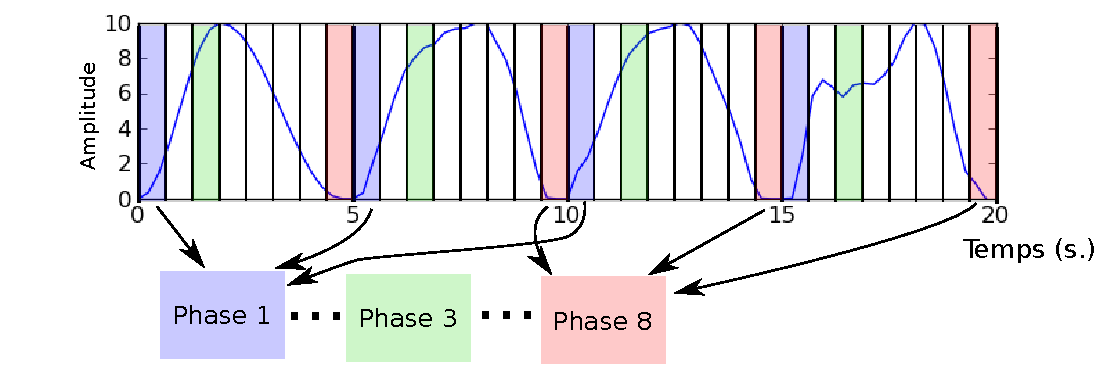
\includegraphics[width=14cm]{images/ET-IM}
	\end{center}
	\caption[Illustration de la synchronisation respiratoire en phase]{Illustration de la synchronisation respiratoire en phase : Le cycle respiratoire acquis est découpé selon la position du signal acquis dans le cycle. Le signal est analysé pour déterminer les débuts et fins de cycles. Chaque cycle est découpé en un nombre déterminé de phases égales.} 
	\label{fig:gatingRespi}
\end{figure}


\begin{figure}[h!]
	\begin{center}
		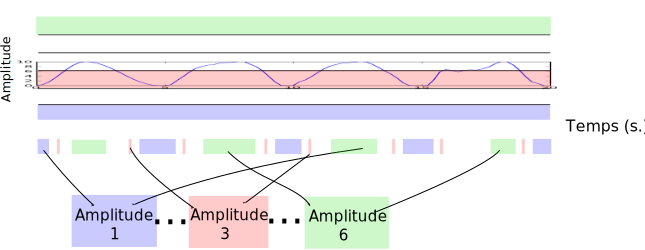
\includegraphics[width=14cm]{images/gatingAmplitude}
	\end{center}
	\caption{Illustration de la synchronisation respiratoire en amplitude : Le cycle respiratoire acquis est découpé selon son amplitude.} 
	\label{fig:gatingRespiAmplitude}
\end{figure}


Cette technique est notamment présentée dans~\cite{nehmeh2002effect}, où le signal respiratoire est estimé par une caméra qui suit un marqueur placé sur le torse du patient (système RPM de Varian Medical Systems). L'étude a été réalisée sur 5 patients volontaires comme suit : un scan de transmission de 3 minutes, suivi d'une acquisition avec correction de 10 minutes, puis d'une acquisition témoin non corrigée de 3 minutes. La décomposition du cycle s'effectue en fonction de la phase. L'auteur annonce une amélioration de l'estimation du volume des tumeurs pouvant aller jusqu'à 34\%, avec une augmentation du $SUV_{max}$ de 160\%. 

Une autre publication~\cite{boucher2004respiratory} utilise un thermomètre détectant l'air chaud émis en début de cycle respiratoire pour réaliser la synchronisation. Les différentes reconstructions issues de l'expérience sont visibles sur la figure~\ref{fig:boucher2004}. Il faut noter que la partie clinique de cette étude a été réalisée sur 10 patients sains, et qu'il n'y a donc pas de mesures de performance de la correction du mouvement sur les lésions. 

\begin{figure}[h!]
	\begin{center}
		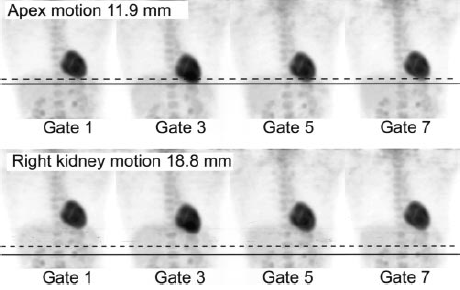
\includegraphics[width=12cm]{images/gatingBoucher2004}
	\end{center}
	\caption[Illustration de l'étendue du mouvement respiratoire sur des images reconstruites ]{Illustration de l'étendue du mouvement respiratoire sur des images reconstruites après synchronisation respiratoire~\cite{boucher2004respiratory}. La rangée du haut montre l'étendue du mouvement de l'apex du coeur, et celle du bas l'étendue du mouvement du rein.} 
	\label{fig:boucher2004}
\end{figure}

Une variante de cette technique ne nécessitant pas de capteur est décrite dans~\cite{nehmeh2003reduction}. Un point faiblement radioactif est fixé au-dessus du torse du patient. Les acquisitions de l'imageur sont ensuite enregistrées par blocs temporels de 1 seconde, et une zone d'intérêt est reconstruite dans chacune des images. Les données reconstruites montrant le point source dans cette zone d'intérêt sont sommées et l'image finale reconstruite. 

Cette technique a été comparée avec celle présentée précédemment~\cite{nehmeh2002effect} basée sur le système RPM de Variant. Ces deux techniques n'ont été testées cliniquement que sur un patient mais ont montré des performances tout à fait semblables (6\% de différence dans les activités et 2\% pour le volume de la lésion).

Cependant, ces techniques n'utilisent pas forcément une carte d'atténuation optimisée pour la position du cycle correspondant aux acquisitions TEP. L'article~\cite{boucher2004respiratory} utilise par exemple une carte d'atténuation obtenue par transmission, qui est une moyenne acquise sur plusieurs cycles respiratoires. Chang et al.~\cite{GuopingChang2010Implementation} estiment la carte d'atténuation à partir d'une image TDM réalisée en respiration libre synchronisée. La phase du cycle respiratoire où l'acquisition TDM a été réalisée est enregistrée, et les données TEP acquises sur tous les cycles à cette phase sont reconstruites (voir exemples figure~\ref{fig:chang2010}). Les résultats présentés sur 13 patients (21 tumeurs) montrent une amélioration du rapport signal sur bruit pouvant aller de -3.4 à 81\% suivant les tumeurs, avec une amélioration moyenne de 26.3\%.

\begin{figure}[h!]
	\begin{center}
		\begin{tabular}{c c}
			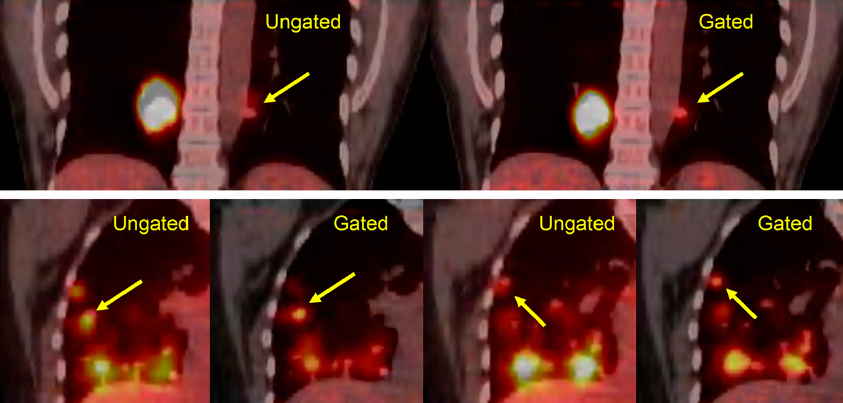
\includegraphics[width=10cm]{images/chang2010}
		\end{tabular}
	\end{center}
	\caption[Images TEP/TDM superposées du poumon]{Images TEP/TDM superposées du poumon reconstruites avec et sans synchronisation respiratoire en utilisant la méthode décrite dans~\cite{GuopingChang2010Implementation}. On peut observer que les tumeurs sont mieux définies et correspondent à l'image TDM qui sert de référence.} 
	\label{fig:chang2010}
\end{figure}

L'inconvénient majeur de ces techniques est qu'elles demandent un temps d'acquisition beaucoup plus long à qualité d'image égale. Si l'on ne conserve que 20\% des évènements détectés, cela signifie qu'il faut augmenter le temps d'acquisition d'un facteur 5 pour obtenir une image de qualité égale. Il n'est donc pas envisageable de mettre en place ces protocoles en routine clinique, car le temps disponible n'est pas suffisant. C'est pour cela que de nombreuses équipes se sont mises à travailler sur une évolution de cette technique, où les images sont acquises en mode synchronisé  puis recalées et sommées pour prendre en compte toute la statistique.

\section{Synchronisation respiratoire avec recalage}
\label{lab:corrPostRecon}

Dans cette section, nous allons détailler la technique consistant à corriger le mouvement en recalant les images reconstruites de chaque phase du cycle respiratoire.

Ces techniques se basent toutes sur une estimation préalable du mouvement respiratoire. Les images de chaque phase sont reconstruites indépendamment, puis recalées sur une phase de référence grâce au champ de mouvement. Enfin, les images déformées sont sommées. La difficulté principale se situe dans l'estimation du champ de mouvement interne lors de la respiration, car ce mouvement est complexe.

Les premières publications décrivant cette technique l'utilisaient notamment pour réaliser de l'imagerie cardiaque en TEP~\cite{klein19973d}. Cette publication démontre la faisabilité du procédé sur un animal en utilisant des techniques de flux optique pour estimer le champ de mouvement. En effet le coeur a l'avantage d'avoir une activité métabolique intense, ce qui rend l'estimation de son mouvement relativement aisée même sur des images avec une faible statistique.




\subsection{Estimation du mouvement respiratoire corps entier}

L'estimation du champ de mouvement interne se fait à l'aide d'une des méthode présentées précédemment en~\ref{lab:estimChamp} et rappelée brièvement :

\subsubsection{Imagerie TEP avec synchronisation respiratoire}
\label{lab:correctionDawood2008}

L'acquisition TEP est réalisée en même temps que l'acquisition du signal respiratoire. Une image est reconstruite par phase du signal respiratoire, puis un algorithme d'estimation de mouvement est utilisé pour calculer le champ de mouvement entre les instants du cycle.

Les premiers algorithmes étaient utilisés en imagerie cardiaque~\cite{klein2002four} avec des transformations simples (affines), puis d'autres algorithmes plus adaptés aux images corps entier ont été utilisés, comme les flux optiques~\cite{dawood2006lung, dawood2006lung}, ou l'interpolation par B-spline~\cite{bai2009regularized}. 


\subsubsection{Imagerie TDM 4D}

Les images TDM 4D peuvent être utilisées pour réaliser l'estimation du mouvement respiratoire au lieu des données TEP. Cela nécessite un temps d'acquisition plus long et augmente la dose d'irradiation reçue par le patient.
Dawood a réalisé plusieurs publications sur le sujet en utilisant le flux optique pour l'estimation du champ de mouvement~\cite{dawood2006lung, dawood2008respiratory}. L'algorithme a été étudié sur des images de patients réels. Une autre publication~\cite{thorndyke2006reducing} indique une amélioration du rapport de contraste sur bruit (CNR) d'un facteur 3 grâce à la correction.


\section{Correction pré-reconstruction}
\label{lab:corrPreRecon}
Les méthodes de correction du mouvement pré-reconstruction modifient les positions des lignes de réponse (LDR) estimée par l'imageur TEP.
Ce recalage des LDR correspond à un déplacement des lignes de réponse dans l'espace du détecteur (voir figure~\ref{fig:recalageLOR}) en fonction du mouvement respiratoire. La limitation principale de ce type de méthode est que le champ de mouvement ne peut pas être élastique.

Cependant, il a été étudié en imagerie du cerveau~\cite{bloomfield2003design}, où il permettait de corriger les mouvements de la tête. Il a été aussi utilisé en imagerie cardiaque TEP~\cite{livieratos2005rigid} en utilisant un champ de mouvement rigide (rotation suivie d'une translation).

Dans les deux cas, les résultats ont montré une nette amélioration des images (voir figure~\ref{fig:ameliorationLOR}).

Dans le cadre du mouvement respiratoire du thorax, l'approche de recalage par LDR a été expérimentée notamment par Frédéric Lamare~\cite{lamare2007respiratory}, mais avec des résultats mitigés. En effet, le champ était approximé par une transformation affine, qui peut difficilement modéliser le mouvement du thorax dans son ensemble. La figure~\ref{fig:lamare2007} montre un profil d'image réalisé pour différents types de corrections. On peut voir que, bien que la correction pré-reconstruction estime correctement la position de la lésion, son activité est beaucoup plus faible que l'activité réelle.

\begin{figure}[h!]
	\begin{center}
		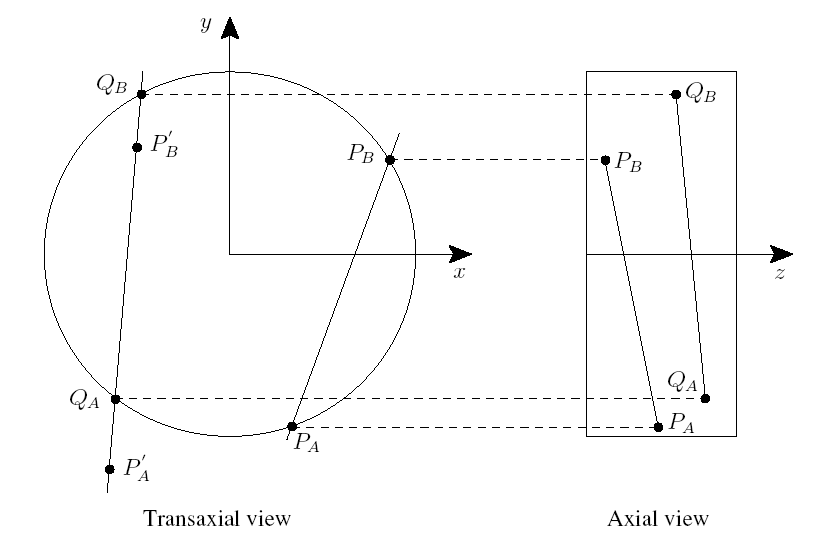
\includegraphics[width=12cm]{images/recalageLOR}
	\end{center}
	\caption[Illustration du recalage des lignes de réponse dans l'espace du détecteur]{Illustration du recalage des lignes de réponse dans l'espace du détecteur : $P_A$ et $P_B$ représentent les positions des détections, $P_{A'}$ et $P_{B'}$ les positions des points corrigés et $Q_A$ et $Q_B$ les détections correspondantes } 
	\label{fig:recalageLOR}
\end{figure}

\begin{figure}[h!]
	\begin{center}
		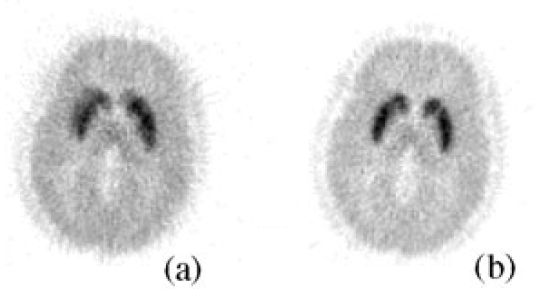
\includegraphics[width=6cm]{images/bloomfield2003design} 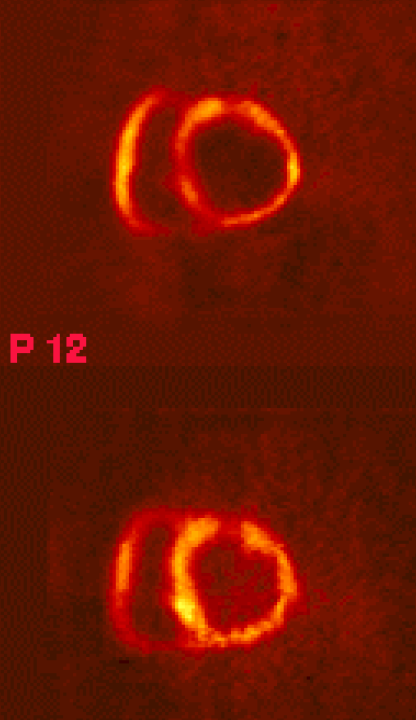
\includegraphics[width=3cm]{images/livieratos2005rigid}
	\end{center}
	\caption[Résultats de l'algorithme de recalage des LDR sur des images de patients]{Résultats de l'algorithme de recalage des LDR sur des images de patients utilisant le radio-traceur [$^{11}$C]raclopride. (a) montre une image non corrigée du mouvement et (b) une image corrigée. On peut noter que les structures internes du cerveau sont beaucoup mieux définies. (c) représente une coupe du c\oe{}ur petit axe non corrigée (en haut) et corrigée (en bas). On peut voir une amélioration de la définition de l'image.} 
	\label{fig:ameliorationLOR}
\end{figure}
 

En effet,~\cite{lamare2007respiratory} réalise une estimation du mouvement, en recalant les images TDM de chaque instant du cycle sur l'image de référence à l'aide d'une transformation affine par maximisation de l'information mutuelle normalisée. Les données sont des simulations réalisées à partir du logiciel GATE~\cite{jan2004gate} et du fantôme NCAT. Des lésions de 7, 11, 15 et 21mm de diamètre ont été placées dans le poumon, avec un contraste de 8. Le champ de mouvement est calculé séparément pour le poumon, le coeur et trois organes sous le diaphragme (foie, estomac, rate).

Ces résultats ont été améliorés par l'utilisation de la technique suivante qui permet la prise en compte d'un mouvement élastique. Les performances comparées des deux méthodes sont présentées dans la section suivante.

\section{Correction pendant la reconstruction}
\label{lab:CorrpendantRecon}
Plusieurs auteurs ont présenté des méthodes permettant de réaliser la correction de mouvement pendant la reconstruction. Qiao et al.~\cite{qiao2006motion} et Lamare et al.~\cite{lamare2007list} ont proposé une méthode de correction du mouvement respiratoire basé sur une modification de la matrice de sensibilité lors de la reconstruction pour prendre en compte le mouvement. Tous les deux utilisent un champ de mouvement élastique estimé en utilisant un champ interpolé par B-splines.

L'algorithme original utilisé est basé sur OPL-EM~\cite{reader2002one} qui organise les données en ``sous-ensemble'' de la même manière que OS-EM~\cite{hudson1994accelerated} mais en utilisant les informations séquentielles présentées en~\ref{lab:modeliste}. Le principe de la reconstruction avec correction du mouvement respiratoire est décrit par la formule suivante :

\label{lab:corrMatSyst}
\begin{equation}
 f^{k+1}=\frac{f^k}{S} \sum_{t=1}^{N} P_t^T \frac{1}{P_t f^k} 
\label{lab:OPLLamara}
\end{equation}

$f^k$ est l'image à l'itération $k$,

$T$ est l'opérateur de transposition

$P_t$ représente la matrice système à l'instant t. Chaque élément $p_{ij}^t$ de cette matrice indique la probabilité de détecter à la ligne de réponse $i$ un évènement généré au voxel $j$ au temps $t$. Cette équation est basée sur l'algorithme OPL-EM présenté en~\ref{lab:OPLEM}. Les informations du champ de mouvement sont contenues dans la matrice $P_t$. $P_t f$ correspond à la projection de l'image $f$ à l'instant $t$.  

$N$ correspond au nombre d'instants temporels considérés.

$S$ est la matrice de sensibilité :

\begin{equation}
 S=\frac{1}{N} \sum_{t=1}^{N} P_t^T M A_t 
\end{equation}

 $A_t$ est la matrice permettant de corriger les effets de l'atténuation au temps $t$ et $M$ est la matrice de normalisation qui compense l'inhomogénéité spatiale de la sensibilité. $A_t$ est estimée à partir des cartes d'atténuation de chaque instant $t$.

L'étude~\cite{lamare2007list} a été réalisée sur des données simulées semblables à celles de l'étude précédente~\cite{lamare2007respiratory}. Il s'agit de simulations réalisées à l'aide du logiciel GATE, d'un cycle respiratoire du modèle NCAT, constitué de 8 instants temporels ainsi qu'une acquisition statique de référence de statistique équivalente à la somme des 8 acquisitions précédentes. Des lésions de 7, 11, 15 et 21 mm de diamètre et d'activité 8 fois plus importante que le fond ont été insérées dans le poumon.
 
Dans la publication, deux variantes de la technique de correction du mouvement respiratoire sont comparées avec la correction par synchronisation respiratoire avec recalage présentée ci-dessus ainsi que la correction pré-reconstruction précisé en~\ref{lab:corrPreRecon}. Des variantes de la méthode nommées ``Reconstruction 1'' et ``Reconstruction 2'' sur la figure correspondent à des différences d'interpolation du champ de mouvement dans la matrice système. Les résultats présentés montrent un clair avantage pour la correction pendant la reconstruction, avec des performances couramment améliorées d'un facteur 2. 

Par exemple, le PRD sur la métrique contraste (équation~\ref{eq:percentAmelioraiton}) pour une lésion de 7mm présente dans la partie haute du poumon est de 28\% pour les images non corrigées, contre 4.4\% pour les images corrigées par la méthode de correction pré-reconstruction et de 1.2\% pour la méthode de reconstruction pendant la reconstruction. De la même manière, pour des lésions de 7mm présentes dans le bas du poumon, les images non corrigées montrent une différence relative de contraste de 32\%, contre 2.63\% pour la correction pré-reconstruction et 1.66\% pour la correction pendant la reconstruction.


\begin{equation}
 \label{eq:percentAmelioraiton}
 \% Am\acute{e}lioration = \left| \frac{Contraste~sur~image~\acute{E}valu\acute{e}e~-Contraste~sur~R\acute{e}f\acute{e}rence}{Contraste~sur~R\acute{e}f\acute{e}rence} \right|
\end{equation}

La figure~\ref{fig:lamare2007} montre un profil de l'interface poumon/foie avec une tumeur pour les différentes techniques de correction. On voit clairement que l'image non corrigée montre un retard dû au flou de mouvement. Ce retard est partiellement corrigé par la correction de mouvement pré-reconstruction, mais le profil de courbe de la méthode de correction du mouvement pendant la reconstruction est celui qui s'approche le plus de la référence.


\begin{figure}[h!]
	\begin{center}
		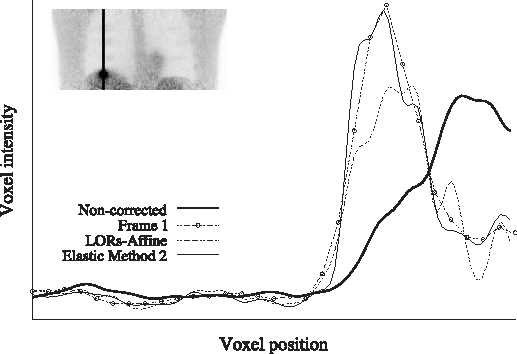
\includegraphics[width=12cm]{images/lamare2007list.pdf}
	\end{center}
	\caption[comparaison des performances des différentes techniques de correction du mouvement sur un profil d'image TEP]{comparaison des performances des différentes techniques de correction du mouvement sur un profil d'image TEP contenant une tumeur placée au niveau du diaphragme. La référence est l'image statique, ``Reconstruction 1'' correspond à la correction pré-reconstruction, et ``Reconstruction 2'' correspond à la correction pendant la reconstruction.} 
	\label{fig:lamare2007}
\end{figure}


\begin{figure}[h!]
	\begin{center}
			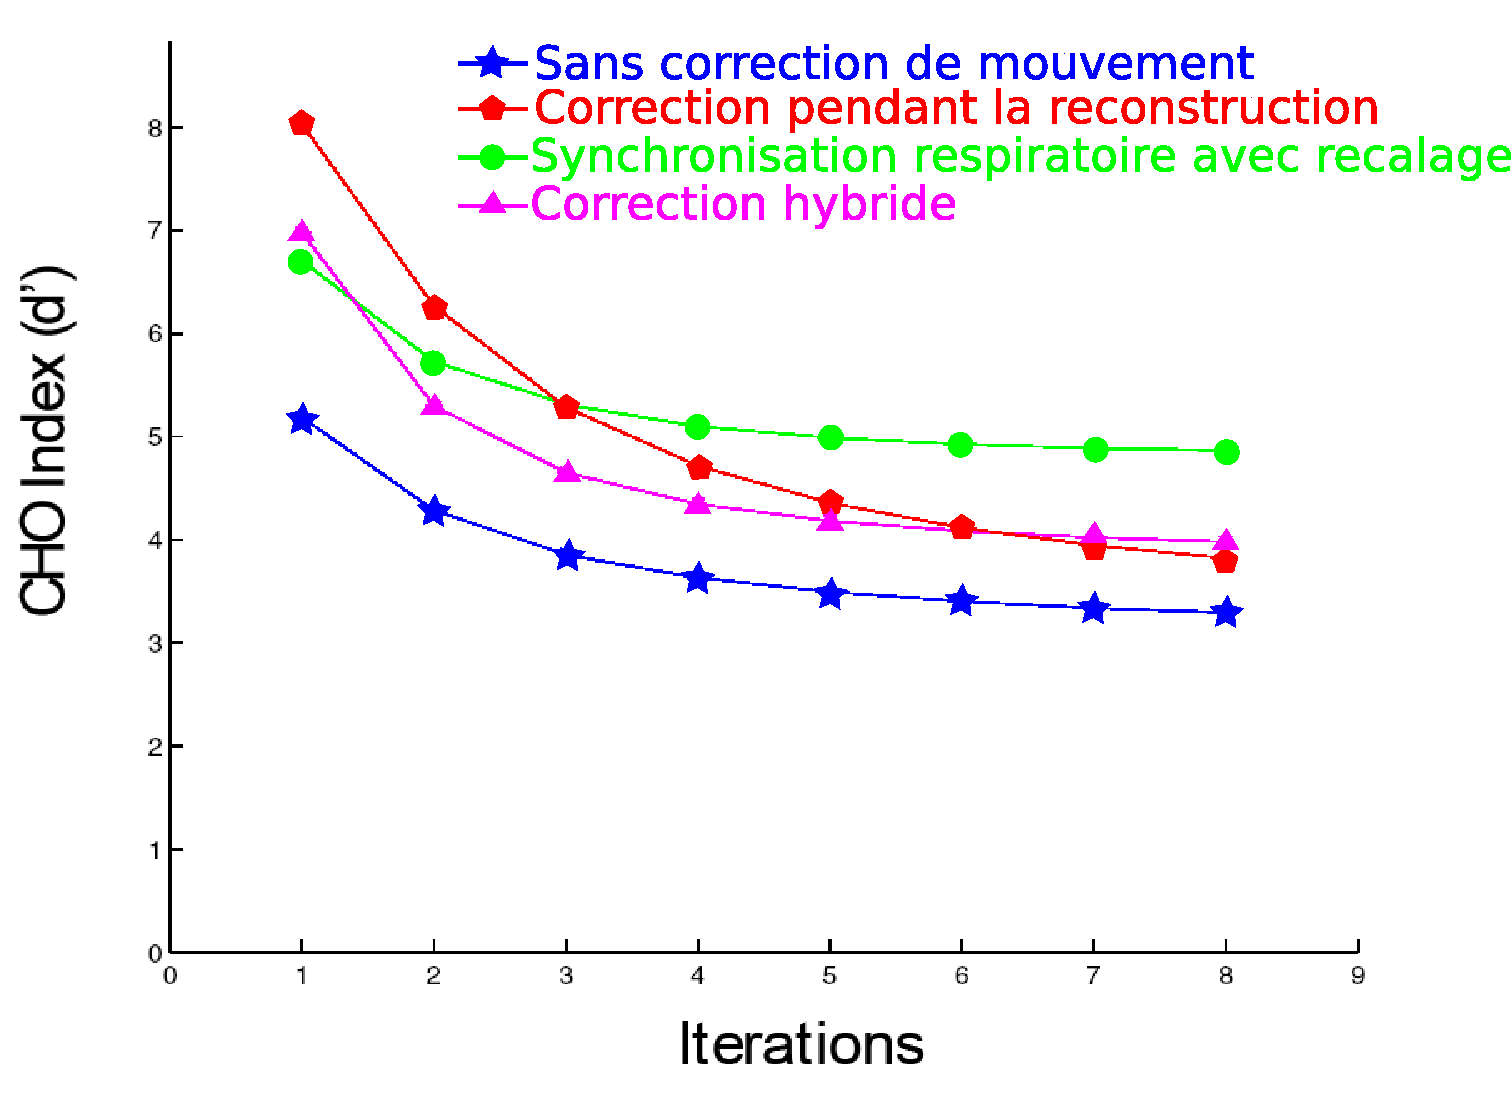
\includegraphics[width=10cm]{images/apportCHO}
	\end{center}
	\caption[Index de CHO pour différentes techniques de correction du mouvement respiratoire en fonction du nombre d'itérations de la reconstruction]{Index de CHO pour différentes techniques de correction du mouvement respiratoire en fonction du nombre d'itérations de l'algorithme de reconstruction. Plus l'indice est important meilleure est la détectabilité. La méthode utilisant la correction post-reconstruction est comparée avec une méthode hybride présentée dans le document en~\ref{lab:evolGating}.} 
	\label{fig:apportCHO}
\end{figure}


 La publication~\cite{Thielemans2006Lesion} présente un système hybride de synchronisation respiratoire avec recalage et de correction de mouvement pendant la reconstruction. Ce système a été développé pour pouvoir isoler l'effet de la sommation des images recalées sur le résultat. Pour cela, les données de chaque instant temporel sont corrigées et reconstruites séparément à l'aide de la formule~\ref{lab:OPLLamara}. Les N images sont ensuite directement sommées pour obtenir l'image corrigée. Les résultats de cette étude, dont la méthode est décrite au paragraphe~\ref{lab:articleThielPres}, sont reportés sur la figure~\ref{fig:apportCHO}. Ils comparent les performances de détection estimées par un observateur numérique (présenté en~\ref{lab:articleThielPres}) sur des images non corrigées du mouvement (symbole étoile), puis sur des image corrigées par les deux modèles de corrections présentés en~\ref{lab:correctionDawood2008} (symbole rond) et~\ref{lab:CorrpendantRecon} (symbole hexagone) et enfin sur sa méthode hybride (symbole triangle). La figure montre que cette technique hybride améliore de manière sensible la détection par rapport aux images non corrigées mais reste inférieure aux deux autres techniques mentionnées pour la mesure de détectabilité, comme présenté dans la figure~\ref{fig:apportCHO}
\label{lab:evolGating}

\section{Déconvolution de l'image}

Cette technique décrite dans~\cite{naqa2006deblurring} utilise une connaissance du mouvement respiratoire acquise à partir d'une image TDM 4D pour déduire un filtrage appelé TLP (\textit{Tumor Location Probability}) qui correspond à la dégradation due au mouvement respiratoire. Un exemple de filtre est représenté sous forme 3D dans la figure~\ref{fig:formeTLP}.

\begin{figure}[h!]
	\begin{center}
		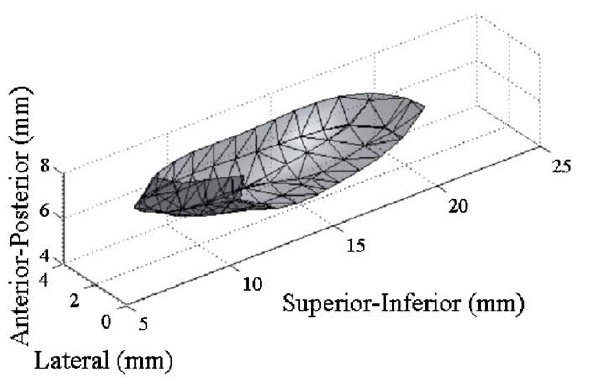
\includegraphics[width=10cm]{images/formeTLP}
	\end{center}
	\caption[Exemple de filtres TLP pour la correction par déconvolution]{Exemple de filtres TLP calculé dans l'article~\cite{naqa2006deblurring} pour la correction par déconvolution, rendu en 3D après tesselation, lissage et normalisation. Il représente la probabilité de présence du centre de la lésion.} 
	\label{fig:formeTLP}
\end{figure}



L'image est déconvoluée pixel par pixel pour corriger les effets du mouvement respiratoire. Cette méthode a été évaluée sur un fantôme physique et des patients réels à l'aide d'un grand nombre de critères provenant pour partie de la TEP (sous-estimation de l'activité de la tumeur, exemples d'images), et pour partie du domaine de la déconvolution (entropie, ``rugosité'').

Les résultats présentés sur la figure~\ref{fig:performanceDeconvolution} montrent une nette amélioration des performances sur des fantômes, pour un déplacement axial simple de 20 mm. L'activité des lésions de fort diamètre ($>$ 20 mm) est correctement récupérée quelque soit l'algorithme utilisé, mais il n'a pratiquement pas d'effets sur les lésions de 1 cm de diamètre.

Ce type de méthode est peu présent dans la littérature par rapport aux autres présentés précédemment. 

\begin{figure}[h!]
	\begin{center}
		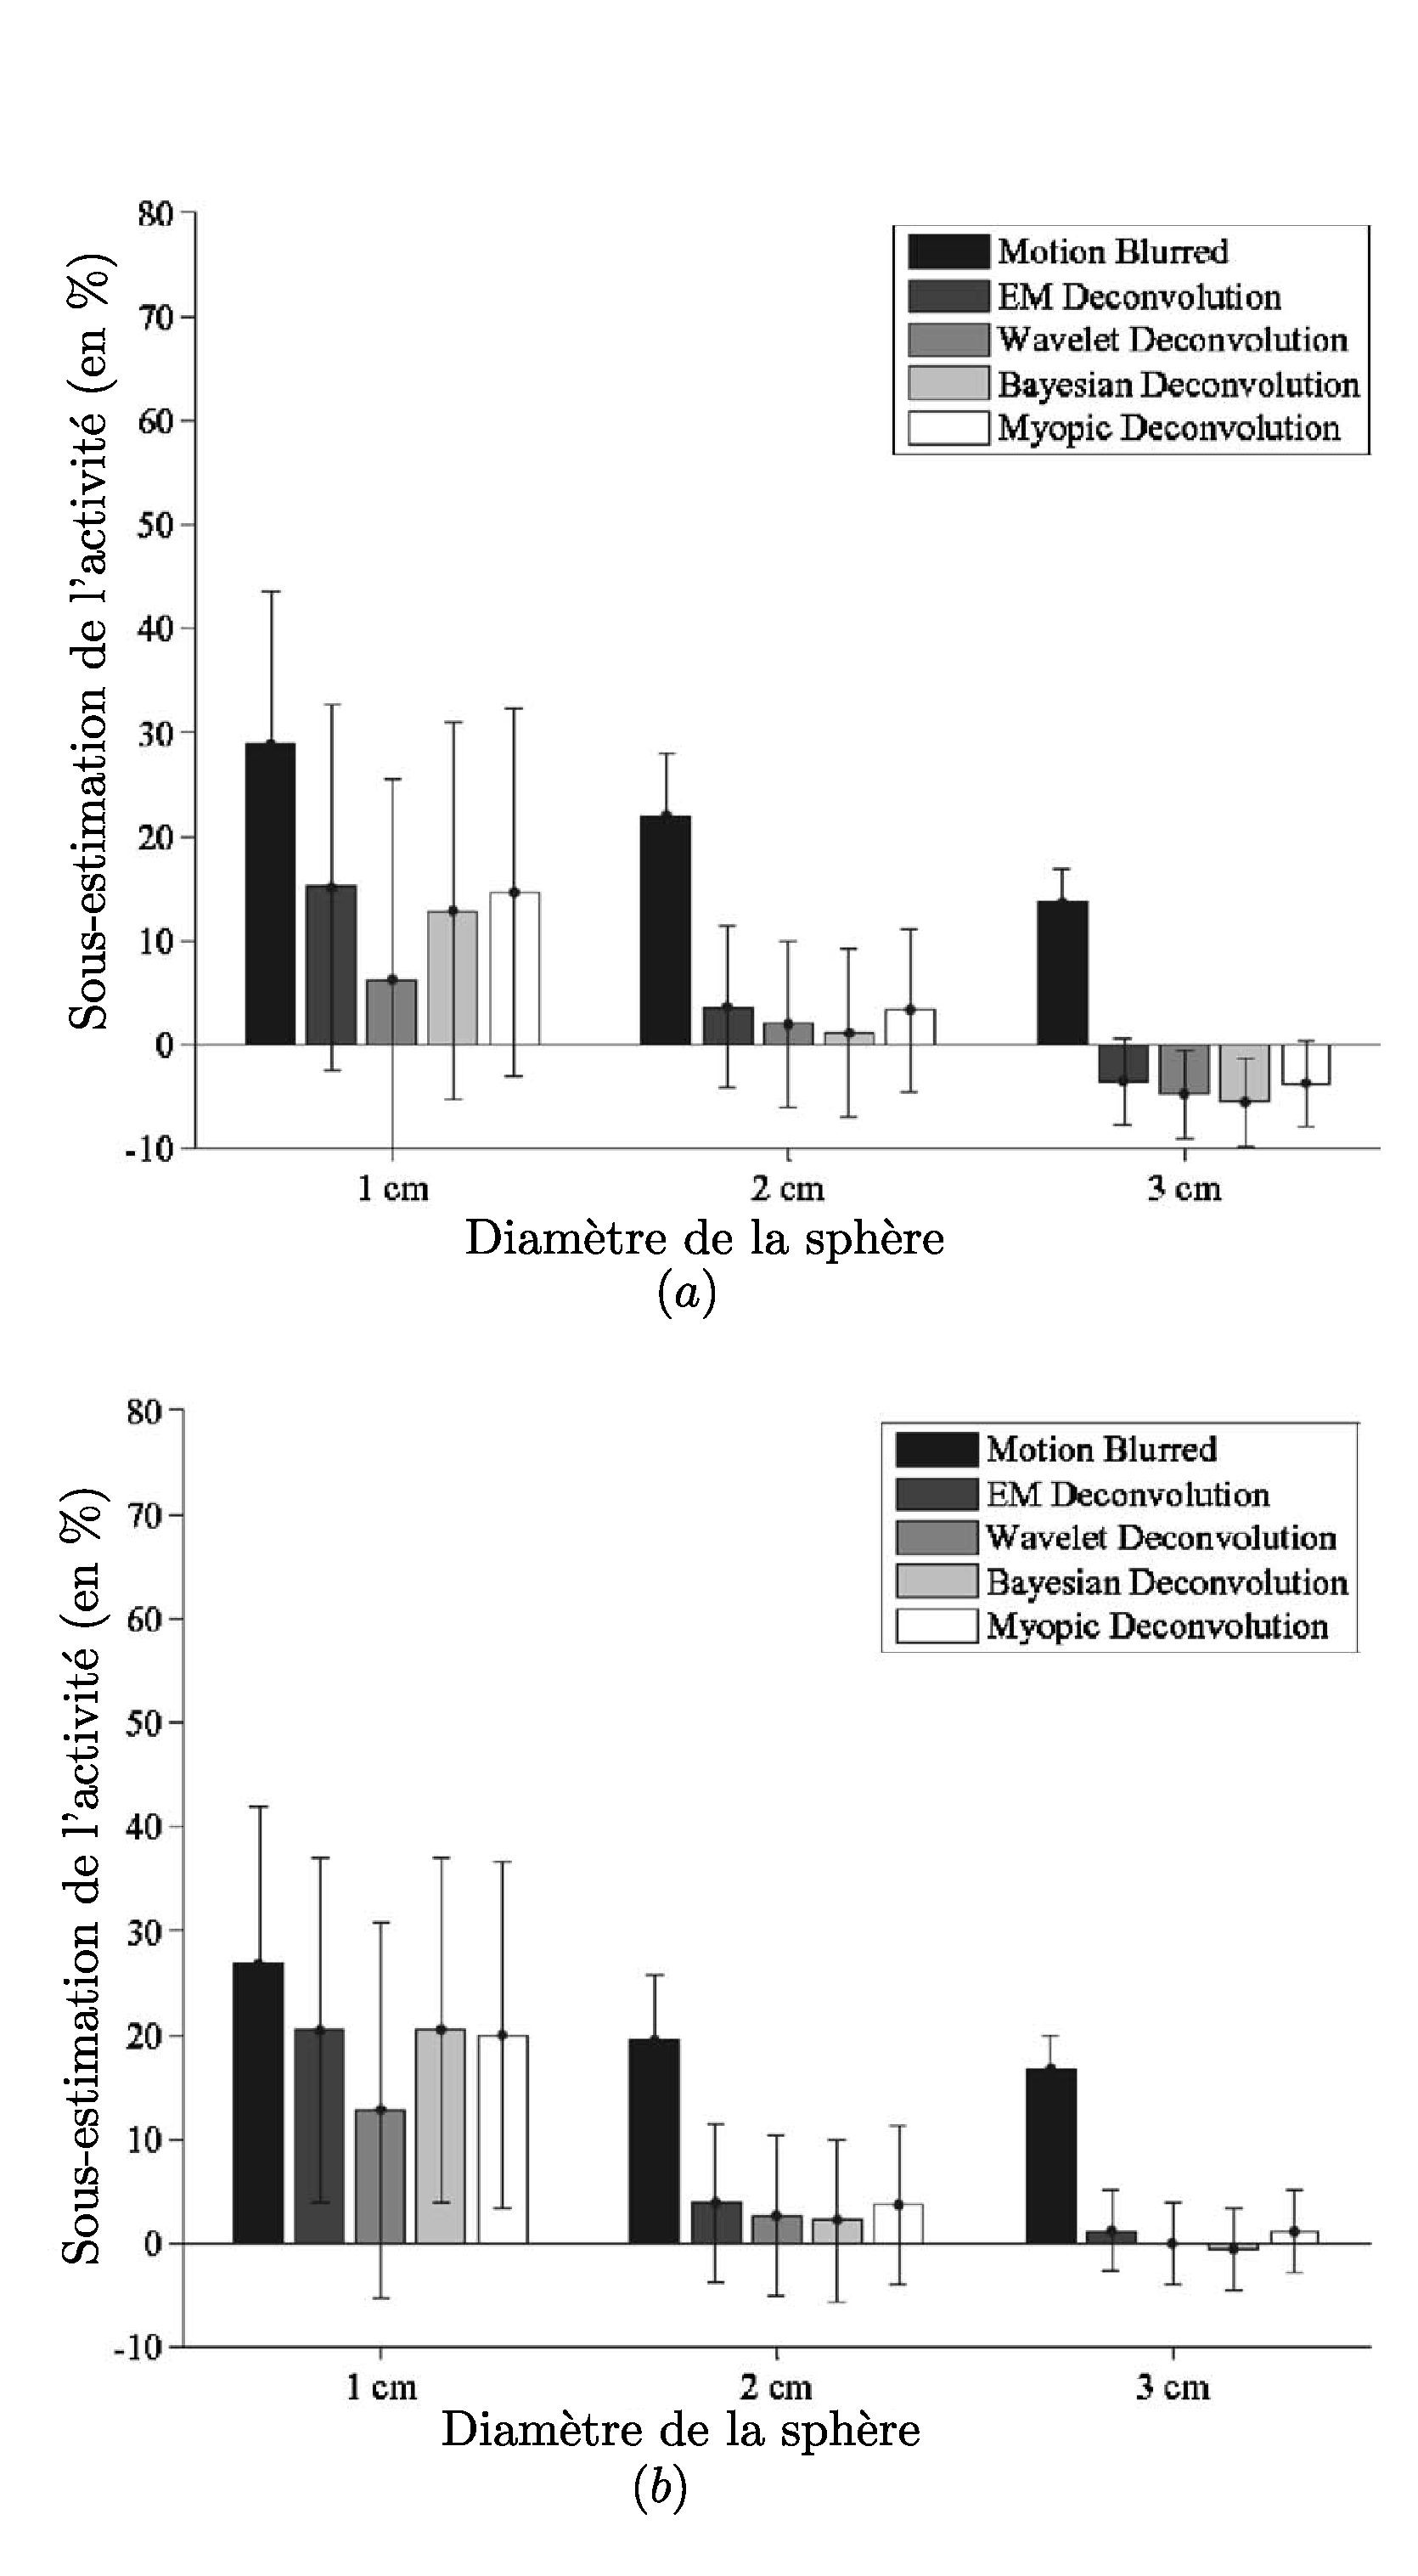
\includegraphics[width=10cm]{images/performanceDeconvolution}
	\end{center}
	\caption[Comparaison de l'erreur de sous-estimation de l'activité des lésions]{Comparaison de l'erreur de sous-estimation de l'activité des lésions en fonction de l'algorithme de déconvolution utilisé sur des fantômes. En a) la lésion a une activité moyenne, tandis qu'en b) l'activité de la lésion est faible par rapport au fond. Le déplacement de la lésion est le même dans les deux cas (2cm).} 
	\label{fig:performanceDeconvolution}
\end{figure}


Un autre article utilisant aussi des algorithmes de déconvolution a été présenté par Wiemker~\cite{wiemker2008combined}. Cependant il ne cherche pas à corriger le mouvement respiratoire sur l'ensemble de l'image mais principalement à améliorer la mesure du SUV sur une lésion. Pour cela, il réalise une estimation de la fonction d'étalement du point (FEP) de l'imageur TEP au niveau de la lésion à l'aide d'un contourage de la lésion réalisé préalablement sur une image TDM. L'estimation de la FEP permet de prendre en compte à la fois les effets du mouvement respiratoire et ceux de la FEP intrinsèque à l'imageur TEP. 

Cependant, cette technique est inapplicable dans notre cas car les lésions doivent être de taille suffisamment importante et homogène pour pouvoir les délimiter de manière fiable sur les images TDM.
